\documentclass[12pt]{article}

\usepackage[utf8]{inputenc}
\usepackage{latexsym,amsfonts,amssymb,amsthm,amsmath}
\usepackage{graphicx}
\usepackage{listings}
\usepackage{xcolor} 

\graphicspath{ {./images/} }

\setlength{\parindent}{0in}
\setlength{\oddsidemargin}{0in}
\setlength{\textwidth}{6.5in}
\setlength{\textheight}{8.8in}
\setlength{\topmargin}{0in}
\setlength{\headheight}{18pt}

\lstset{
  mathescape,
  backgroundcolor=\color{gray!10},  
  basicstyle=\ttfamily,
  columns=fullflexible,
  breakatwhitespace=false,      
  breaklines=true,                
  captionpos=b,                    
  commentstyle=\color{green}, 
  extendedchars=true,              
  frame=single,                   
  keepspaces=true,             
  keywordstyle=\color{blue},      
  language=c++,                 
  numbers=none,                
  numbersep=5pt,                   
  numberstyle=\tiny\color{blue}, 
  rulecolor=\color{gray},        
  showspaces=false,               
  showstringspaces=false,
  showtabs=false,                 
  stepnumber=5,                  
  stringstyle=\color{red},   
  tabsize=3,                      
  title=\lstname                
}



\title{Home assignment for Computer Network EDA387}
\author{Group 24}

\begin{document}

\maketitle

\vspace{0.5in}

\paragraph{Problem}

% Problem statement or description should be placed in there
Let $P = \{p_0, \ldots, p_{n-1}\}$ be $n$ processors on a directed ring, 
as considered by Dijkstra in his self-stabilizing token circulation algorithm. 
In this model, processors are \emph{semi-uniform}, i.e., there is one distinguished 
processor $p_0$ that runs a different program than all other processors, 
but processors do not have unique identifiers. 

Recall that in Dijkstra’s directed ring, each processor $p_i$ can only read from 
$p_{(i-1)\bmod n}$'s shared variables, and each processor can use shared variables 
of constant size. 

For each of the following questions, please provide:
\begin{itemize}
  \item a clearly written pseudo-code of the algorithm, 
  \item a definition of the set of legal executions, 
  \item a correctness proof with all necessary arguments to convince the reader 
        that the algorithm is both correct and self-stabilizing. 
\end{itemize}

Prove your claims.

\subsection*{Question 1}

% Question 1 statement should be placed in there, modify the {} subsection to match.
% \includegraphics[scale=set_to_fit_with_space]{relative_or_absolute_path_is_fine}

The vertex-coloring problem is crucial for resource allocation, scheduling,
and network topology control tasks. It involves assigning colors to the 
processors (aka vertices of a graph) so that no two neighboring processors 
share the same color. Specifically, each $p_i \in P$ must be assigned a 
color $x_i$, such that $x_i \neq x_{(i-1) \bmod n}$. The main complexity 
measure is the total number of colors $k$ used to color the network. 
Design a deterministic self-stabilizing vertex-coloring algorithm that 
always provides an optimal solution (after stabilization). Assume that $n$ 
is known.

\bigskip

\begin{proof}

% Place your work in here

% Consider to use textbf or textit to highlight important parts. Using itemzine or enumerate to structure your work is also a good idea.

Let consider this pseudo-code block for the vertex-coloring problem.

\begin{lstlisting}    
01: $P_0$: do forever

02:      if $x_0$ % 2 $==$ 0: then $x_0$ := 1;

03:      else $x_0$ := 2;

04: $P_i$ $(i \neq 0)$: do forever

05:      if $x_i$ $==$ $x_{(i - 1) \bmod n}$: then $x_i$ := ($x_{(i - 1) \bmod n}$ + 1) $\bmod$ 2
\end{lstlisting}

The block above illustrated the process of assigning color for all vertexs. For this algorithm, the complexity
depends on the total number of processors. If it is even, it needs at least 2 different colors, but if it is odd, 
it needs at least 3 colors. Because if only use 2 color for the odd number of processors, the 
root and its right neighbor will have the same color after the "correction flood", as shown in the
figure. We can even use more color than the number of processors (Pigeonhole) but this focuses on the least complexity.
The $\bmod 2$ is used for assigning color to non-root processors as we only use at least colors for this process. 

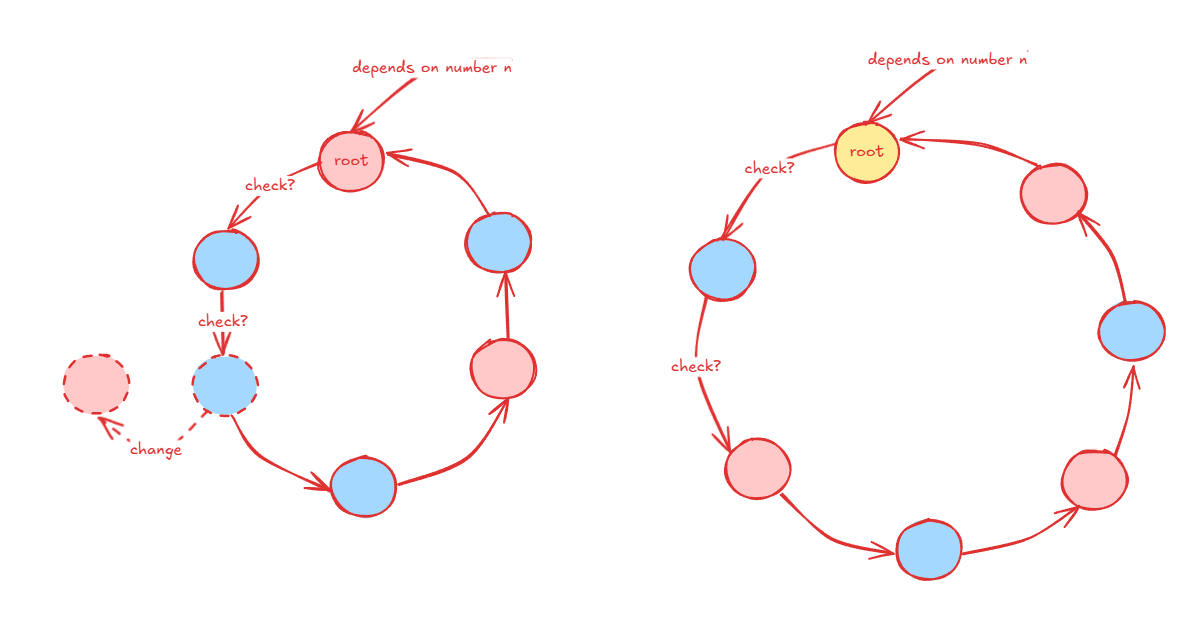
\includegraphics[scale=0.35]{ring-color-self-stablize.png}

\begin{itemize}
    \item \textbf{Legal executions} each processors can change or remain the same each round. The root processor is assigned
    a value at start.
    \item \textbf{Correctness} this algorithm proves that, any two neighboring processors must have different color.
    As in line 05, take an example that the $P_3$ (where i is not equal to 0) has value of $x_i$ $=$ 1. The condition is 
    now met and it forces $P_4$ to take another value for its $x_4$, which must be $(x_3 + 1) \bmod 2 = 0$. All non-root processor 
    changes its value to a value in range $\{0,1\}$. On the other hand, the root processor itself have a mechanism to ensure 
    after an asynchronous cycle, where every processors take at least 1 round in the \textbf{do forever} loop, it must not have
    same value with its neighbors. The value is assigned to root, depends on the total number of processors. Therefore, it is easy
    to notice that, in the case of odd, if just use 2 color, the last processor will have the same color as root, triggering another
    round of color assigning, so that in this case, root must have a distinguished color (that can not be achieved with $\bmod 2$)
    \item \textbf{Self-stabilizing} the system always reach the correct state because of the root is assigned a defined value at 
    the start. While the others can react to the "stabilizing" by changing state depends on its comparison with neighbor's state.
    In addition, because this algorithm flows to just one direction and begins from a fixed point (the root, with user's defined color/state)
    the system can not get in a loop of be stuck in some step, thus guarantes \textbf{self-stabilization}.
\end{itemize}
\end{proof}

% Add more subsection if there is more than one question.
\subsection*{Question 2}

The maximum matching problem is essential in optimizing resource allocation,
communication, and network design. It involves finding the largest possible set
of pairs of neighboring processors, aka edges, in the network, such that no two pairs
share a processor. Specifically, a matching $M \subseteq \{(p_i, p_{(i-1) \bmod n}) : p_i \in P\}$ 
is a subset of neighboring pairs, such that no two neighboring pairs in $M$ share a processor, 
i.e., for any two neighboring pairs $(p_i, p_{(i-1) \bmod n})$ and $(p_j, p_{(j-1) \bmod n})$ in $M$, 
$p_{(i-1) \bmod n} \neq p_j$ and $p_{(j-1) \bmod n} \neq p_i$. The goal is to find a matching 
$M$ to maximize the number of neighboring pairs in $M$. Design a deterministic 
self-stabilizing maximum matching algorithm that always provides an optimal 
solution (after stabilization). Assume that $n$ is known.

\bigskip

\begin{proof}

Let begin with the process to form the maximum numbers of pairs.

\begin{lstlisting}
01: $P_0$: do forever
02:         if not $matched$ $AND$ then:
03:           $token$
04:           if $P_{(i-1) \bmod n}$ is not $matched$ then:
05:              matched: = true
06:              pass $token$ to $P_{(i+1) \bmod n}$
07: $P_i$: do forever
08:         if $token$ then:
09:             if $P_{(i-1) \bmod n}$ is not $matched$ and $P_i$ is not $matched$ then:
10:               matched: = true
11:               pass $token$ to $P_{(i+1) \bmod n}$
12:             else:
13:               pass $token$ to $P_{(i+1) \bmod n}$
\end{lstlisting}

The pseudo-code block above illustrates the process to form pair between 2 neighboring processors. This process is
triggered by the root processor. The $token$ acts as an authorized token for the execution of each processor. Only 
the root can issued it while the others simply received and passed it. Each processor will check the predecessor to
determine if it is suitable for a $matched$ condition. If the predecessor is already $matched$, it simply passes 
$token$ to the next process.

\begin{itemize}
  \item \textbf{Legal execution} each processor other than the root can only act if it has the $token$. Moreover,
  if the condition is met (both the processor and its predecessor are available for a $matched$) the pair will be
  formed. On the other hand, it simple passes the $token$ to another processor.
  \item \textbf{Correctness} this process is initialized by the root processor (which issues the $token$). The $token$
  is a mechanism to ensure only a processor can act at a time to avoid race condition. 
  \item \textbf{Self-stabilization} from any initial state (even arbitrary one), the $token$ always visit all the processors
  and "fix" the matching if needed. This leads to a legal maximum matching in a finite time.
  \item \textbf{Maximum} if n is even, all processor will have its matched, otherwise, there is only 1 processor left. This
  ensures the maximum matching in this ring.
\end{itemize}
\end{proof}

\vspace{3in}

\end{document}
% vim: set ts=4 sw=4 et:                